         \chapter{States of matter and the kinetic molecular theory}
    \setcounter{figure}{1}
    \setcounter{subfigure}{1}
    \label{3fc6acf7f608d0b0e2d136d6a7710402}
         \section{ States of matter}
    \nopagebreak
            \label{m38736} $ \hspace{-5pt}\begin{array}{cccccccccccc}   \end{array} $ \hspace{2 pt}\raisebox{-5 pt}{
\includegraphics[width=0.5cm]{col11305.imgs/summary_www.png}} {(section shortcode: P10014 )} \par 
\label{m38736*cid1}
            \subsection{ Introduction}
            \nopagebreak
\label{m38736*id802341}In this chapter we will explore the states of matter and then look at the kinetic molecular theory. Matter exists in three states: solid, liquid and gas. We will also examine how the kinetic theory of matter helps explain boiling and melting points as well as other properties of matter.\par 
\label{m38736*cid2}
            \subsection{ States of matter}
            \nopagebreak
\label{m38736*id324876121}All matter is made up of particles. We can see this when we look at diffusion.
\Definition{Diffusion}{Diffusion is the movement of particles from a high concentration to a low concentration.} 
Diffusion can be seen as a spreading out of particles resulting in an even distribution of the particles. You can see diffusion when you place a drop of food colouring in water. The colour slowly spreads out through the water. If matter were not made of particles then we would only see a clump of colour when we put the food colouring in water, as there would be nothing that could move about and mix in with the water. The composition of matter will be looked at in What are the objects around us made of? (Chapter~11). 
\par 
\label{m38736*id10987324}\textbf{Diffusion} is a result of the constant thermal motion of particles. In  we will talk more about the thermal motion of particles. 
\par 
\label{m38736*id0128031}In 1828 Robert Brown observed that pollen grains suspended in water moved about in a rapid, irregular motion. This motion has since become known as \textbf{Brownian motion}. Brownian motion is essentially diffusion of many particles.
\par 
\label{m38736*id48327}Matter exists in one of three states, namely solid, liquid and gas. Matter can change between these states by either adding heat or removing heat. This is known as a change of state. As we heat an object (e.g. water) it goes from a solid to a liquid to a gas. As we cool an object it goes from a gas to a liquid to a solid.
The changes of state that you should know are:
\label{m38736*id02341}\begin{itemize}[noitemsep]
\item \textbf{Melting} is the process of going from solid to liquid.
\item \textbf{Boiling (or evaporation)} is the process of going from liquid to gas.
\item \textbf{Freezing} is the process of going from liquid to solid.
\item \textbf{Condensation} is the process of going from gas to liquid.
\item \textbf{Sublimation} is the process of going from a solid to a gas. \end{itemize}
A solid has a fixed shape and volume. A liquid takes on the shape of the container that it is in. A gas completely fills the container that it is in. See for more on changes of state.
\par \label{m38736*eip-957}If we know the melting and boiling point of a substance then we can say what state (solid, liquid or gas) it will be in at any temperature. \par \label{m38736*eip-232}
            \begin{fexperiment}{States of matter}{
            \nopagebreak
            \label{m38736*eip-860}\noindent{}\textbf{Aim}
To investigate the heating and cooling curve of water. \\
\par 
\label{m38736*eip-861}\noindent{}\textbf{Apparatus} \\
\begin{minipage}{0.2\textwidth}
\begin{itemize}
 \item beakers
 \item ice
 \item bunsen burner
 \item thermometer
 \item water
\end{itemize}
\end{minipage}
\begin{minipage}{0.8\textwidth}
\begin{figure}[H]
 \begin{center}
\scalebox{0.8}
{
  \begin{pspicture}(-5,-5)(5,5)
\psset{unit=1cm}
%\psgrid(0,0)(-5,-5)(5,5)
\newpsstyle{aspectLiquide1}{linestyle=none,fillstyle=solid,fillcolor=GrisTresClair}
%\uput[r](3.5,1){\large{boiling water}}
%\psline[linewidth=0.04]{->}(3.55,1)(2.6,1)
%\uput[r](3.5,3){\large{metal spoon}}
%\psline[linewidth=0.04]{->}(3.55,3)(3,3)
\psline[linewidth=0.1](-4.7,-2)(-2,2)
\rput(-4,0){\pstTubeEssais[glassType=becher,niveauLiquide1=20,solide={\pstGrenailleZinc[100]}]}
\psline[linewidth=0.04]{<-}(-2.34,1.5)(-1.5,1.5)
\uput[r](-1.5,1.5){\large{Thermometer}}
\psline[linewidth=0.04]{<-}(-3,-1)(-1.5,-1)
\uput[r](-1.5,-1){\large{Beaker}}
\psline[linewidth=0.04]{<-}(-3.5,-1.5)(-1.5,-1.5)
\uput[r](-1.5,-1.5){\large{Ice}}
\psline[linewidth=0.1](1.4,-2)(4,2)
\rput(2,0){\pstTubeEssais[glassType=becher,niveauLiquide1=30]}
\psline[linewidth=0.04]{<-}(3.7,1.5)(4.5,1.5)
\uput[r](4.5,1.5){\large{Thermometer}}
\psline[linewidth=0.04]{<-}(3,-1)(4.5,-1)
\uput[r](4.5,-1){\large{Beaker}}
\psline[linewidth=0.04]{<-}(2.5,-1.5)(4.5,-1.5)
\uput[r](4.5,-1.5){\large{Water}}
\end{pspicture}
}
 \end{center}

\end{figure}
\end{minipage} \\

\label{m38736*eip-862}\noindent{}\textbf{Method}
\label{m38736*id9872}\begin{itemize}[noitemsep]
            \item Place some ice in a beaker\item Measure the temperature of the ice and record it.\item After 1 minute measure the temperature again and record it. Repeat every minute, until at least 1 minute after the ice has melted.\item Heat some water in a beaker until it boils. Measure and record the temperature of the water.\item Remove the water from the heat and measure the temperature every 1 minute, until the beaker is cool to touch\end{itemize}

\\
\par 
\pagebreak
\label{m38736*eip-282}
% \begin{tabular}{cc}
% 	\hspace*{-50pt}\raisebox{-8 mm}{\hspace{-0.2in}
\includegraphics[width=0.5in]{col11305.imgs/pstip2.png} } & 
% 	\begin{minipage}{0.85\textwidth}
% 	\begin{note}
      \Warning {Be careful when handling the beaker of hot water. Do not touch the beaker with your hands, you will burn yourself.}
% 	\end{note}
% 	\end{minipage}
% 	\end{tabular}
	\par
      \label{m38736*eip-863}\noindent{}\textbf{Results}Record your results in the following table:
    % \textbf{m38736*uid434}\par
          \begin{table}[H]
    % \begin{table}[H]
    % \\ '' '0'
        \begin{center}
      \label{m38736*uid434}
    \noindent
    \tabletail{%
        \hline
        \multicolumn{4}{|p{\mytableboxwidth}|}{\raggedleft \small \sl continued on next page}\\
        \hline
      }
      \tablelasttail{}
      \begin{xtabular}[t]{|l|l|l|l|}\hline
                \textbf{Temperature of ice}
               &
                \textbf{Time (s)}
               &
                \textbf{Temperature of water}
               &
                \textbf{Time (s)}
              % make-rowspan-placeholders
     \tabularnewline\cline{1-1}\cline{2-2}\cline{3-3}\cline{4-4}
      %--------------------------------------------------------------------
         &
         &
         &
        % make-rowspan-placeholders
     \tabularnewline\cline{1-1}\cline{2-2}\cline{3-3}\cline{4-4}
      %--------------------------------------------------------------------
         &
         &
         &
        % make-rowspan-placeholders
     \tabularnewline\cline{1-1}\cline{2-2}\cline{3-3}\cline{4-4}
      %--------------------------------------------------------------------
         &
         &
         &
        % make-rowspan-placeholders
     \tabularnewline\cline{1-1}\cline{2-2}\cline{3-3}\cline{4-4}
      %--------------------------------------------------------------------
         &
         &
         &
        % make-rowspan-placeholders
     \tabularnewline\cline{1-1}\cline{2-2}\cline{3-3}\cline{4-4}
      %--------------------------------------------------------------------
         &
         &
         &
        % make-rowspan-placeholders
     \tabularnewline\cline{1-1}\cline{2-2}\cline{3-3}\cline{4-4}
      %--------------------------------------------------------------------
    \end{xtabular}
      \end{center}
\end{table}
    \par
Plot a graph of temperature against time for the ice melting and the boiling water cooling. 
\par 
\label{m38736*eip-864}\noindent{}\textbf{Discussion and conclusion}Discuss your results with others in your class. What conclusions can you draw? You should find that the temperature of the ice increases until the first drops of liquid appear and then the temperature remains the same, until all the ice is melted. You should also find that when you cool water down from boiling, the temperature remains constant for a while, then starts decreasing. 
\par \label{m38736*eip-25}In the above experiment, you investigated the heating and cooling curves of water. We can draw heating and cooling curves for any substance. A heating curve of a substance gives the changes in temperature as we move from a solid to a liquid to a gas. A cooling curve gives the changes in temperature as we move from gas to liquid to solid. An important observation is that as a substance melts or boils, the temperature remains constant until the substance has changed state. This is because all the heat energy goes into breaking or forming the forces between the molecules. \par \label{m38736*eip-166}The above experiment is one way of demonstrating the changes of state of a substance. Ice melting or water boiling should be very familiar to you. \par }
\end{fexperiment}
\label{m38736**end}
         \section{ Properties of matter}
    \nopagebreak
            \label{m38734} $ \hspace{-5pt}\begin{array}{cccccccccccc}   
\includegraphics[width=0.75cm]{col11305.imgs/summary_video.png} &   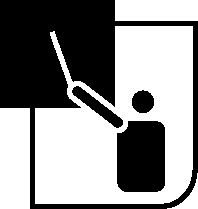
\includegraphics[width=0.75cm]{col11305.imgs/summary_presentation.png} &   \end{array} $ \hspace{2 pt}\raisebox{-5 pt}{} {(section shortcode: P10015 )} \par 
    \label{m38734*cid6}
            \subsection{ The Properties of Matter }
            \nopagebreak
            \label{m38734*id309103}Let us now look at what we have learned about chemical 
bonds, intermolecular forces and the kinetic theory of matter, and see whether 
this can help us to understand some of the macroscopic properties of materials.
\par 
      \label{m38734*id309108}\begin{enumerate}[noitemsep, label=\textbf{\arabic*}. ] 
            \label{m38734*uid43}\item \textbf{Melting point}
\par
            \label{m38734*fhsst!!!underscore!!!id276}\begin{definition}
	  \begin{tabular*}{15 cm}{m{15 mm}m{}}
	\hspace*{-50pt}  
\includegraphics[width=0.5in]{col11305.imgs/psflag2.png}   & \Definition{   \label{id2412224}\textbf{ Melting point }} { \label{m38734*meaningfhsst!!!underscore!!!id276}
The temperature at which a \textsl{solid} changes 
its phase or state to become a \textsl{liquid}. The 
process is called melting and the reverse process (change in phase from liquid 
to solid) is called \textbf{freezing}. 
 } 
      \end{tabular*}
      \end{definition}
In order for a solid to melt, the energy of the particles 
must increase enough to overcome the bonds that are holding the particles 
together. It makes sense then that a solid which is held together by strong 
bonds will have a \textsl{higher} melting point 
than one where the bonds are weak, because more energy (heat) is needed to break 
the bonds. In the examples we have looked at metals, ionic solids and some 
atomic lattices (e.g. diamond) have high melting points, whereas the melting 
points for molecular solids and other atomic lattices (e.g. graphite) are much 
lower. Generally, the intermolecular forces between molecular solids are 
\textsl{weaker} than those between ionic and 
metallic solids.
\label{m38734*uid44}\item \textbf{Boiling point}
\par
            \label{m38734*fhsst!!!underscore!!!id282}\begin{definition}
	  \begin{tabular*}{15 cm}{m{15 mm}m{}}
	\hspace*{-50pt}  
\includegraphics[width=0.5in]{col11305.imgs/psflag2.png}   & \Definition{   \label{id2412302}\textbf{ Boiling point }} { \label{m38734*meaningfhsst!!!underscore!!!id282}
The temperature at which a \textsl{liquid} changes 
its phase to become a \textsl{gas}. The process is 
called evaporation and the reverse process is called condensation 
 } 
      \end{tabular*}
      \end{definition}
When the temperature of a liquid increases, the average 
kinetic energy of the particles also increases and they are able to overcome 
the bonding forces that are holding them in the liquid. When boiling point is 
reached, \textsl{evaporation} takes place and some 
particles in the liquid become a gas. In other words, the energy of the 
particles is too great for them to be held in a liquid anymore. The stronger the 
bonds within a liquid, the higher the boiling point needs to be in order to 
break these bonds. Metallic and ionic compounds have high boiling points while 
the boiling point for molecular liquids is lower.
The data in Table 2.2 below may help you to understand some of 
the concepts we have explained. Not all of the substances in the table are 
solids at room temperature, so for now, let's just focus on the \textsl{boiling points} for each of these substances. What do 
you notice?
    % \textbf{m38734*uid45}\par
\begin{table}[H]
    % \begin{table}[H]
    % \\ 'id2881467' '1'
 \begin{center}
      \label{m38734*uid45}
\begin{tabular}{|l|l|l|}\hline
\textbf{Substance} & \textbf{Melting point (${}^{\ensuremath{{\,}^{\circ}}}\mathrm{C}$)} & \textbf{Boiling point (${}^{\ensuremath{{\,}^{\circ}}}\mathrm{C}$)} \\ \hline
Ethanol (${\mathrm{C}}_{2}{\mathrm{H}}_{6}\mathrm{O}$) & $-114,3$ & $78,4$ \\ \hline
Water                    & $0$      & $100$  \\ \hline
Mercury                                                & $-38,83$ & $356,73$ \\ \hline
Sodium chloride & $801$ & $1465$ \\ \hline
    \end{tabular}
      \end{center}
    \begin{caption}{The melting and boiling points for a number of substances}\end{caption}
\end{table}

    \par
You will have seen that substances such as ethanol, with relatively weak 
intermolecular forces, have the lowest boiling point, while substances with 
stronger intermolecular forces such as sodium chloride and mercury, must be 
heated much more if the particles are to have enough energy to overcome the 
forces that are holding them together in the liquid. See the section (Section~2.2.1.1: Exercise: Forces and boiling point ) below for a further exercise on boiling point. \label{m38734*uid973}\item \textbf{Density and viscosity}\label{m38734*eip-726}
\par Density and viscosity is not in CAPS - Included for Completeness
	\par
%       \label{m38734*fhsstid83}\begin{definition}
% 	  \begin{tabular*}{15 cm}{m{15 mm}m{}}
% 	\hspace*{-50pt}  
\includegraphics[width=0.5in]{col11305.imgs/psflag2.png}   & 
\Definition{ \label{id2412522} Density } { \label{m38734*meaningfhsstid83}Density is a measure of the mass of a substance per 
unit volume. } 
%       \end{tabular*}
%       \end{definition}
The density of a solid is generally higher than that of a liquid because the particles are held much more closely together and therefore there 
are more particles packed together in a particular volume. In other words, there is a greater mass of the substance in a particular volume. In general, density increases as the strength of the intermolecular forces increases. \vspace{\rubberspace}\par
%         \label{m38734*fhsstid84}\begin{definition}
% 	  \begin{tabular*}{15 cm}{m{15 mm}m{}}
% 	\hspace*{-50pt}  
\includegraphics[width=0.5in]{col11305.imgs/psflag2.png}   & 
\Definition{   \label{id2412552} Viscosity } { \label{m38734*meaningfhsstid84}Viscosity is a measure of how resistant a liquid is to 
flowing (in other words, how easy it is to pour the liquid from one container to 
another). } 
%       \end{tabular*}
%       \end{definition}
 Viscosity is also sometimes described as the 'thickness' of a fluid. 
Think for example of syrup and how slowly it pours from one container into 
another. Now compare this to how easy it is to pour water. The viscosity of 
syrup is greater than the viscosity of water. Once again, the stronger the 
intermolecular forces in the liquid, the greater its viscosity.
\end{enumerate}
\label{m38734*eip-473}It should be clear now that we can explain a lot of 
the \textbf{macroscopic properties} of matter (i.e. 
the characteristics we can see or observe) by understanding their \textbf{microscopic structure} and the way in which the atoms 
and molecules that make up matter are held together.\par \label{m38734*secfhsst!!!underscore!!!id289}
            \begin{exercises}{Forces and boiling point}{
            \nopagebreak
            \label{m38734*uid9732}The table below gives the molecular formula and the boiling point 
for a number of organic compounds called \textsl{alkanes} (more on these compounds in grade 12). Refer 
to the table and then answer the questions that follow.
    % \textbf{m38734*id309695}\par
          \begin{table}[H]
    % \begin{table}[H]
    % \\ '' '0'
        \begin{center}
      \label{m38734*id309695}
      \begin{tabular}{|l|l|l|}\hline
\textbf{Organic compound} & \textbf{Molecular formula} & \textbf{Boiling point (${}^{\ensuremath{{\,}^{\circ}}}\mathrm{C}$)} \\ \hline
        Methane & ${\mathrm{CH}}_{4}$ & $-161.6$ \\ \hline
        Ethane & ${\mathrm{C}}_{2}{\mathrm{H}}_{6}$ & $-88.6$ \\ \hline
        Propane & ${\mathrm{C}}_{3}{\mathrm{H}}_{8}$ & $-45$ \\ \hline
        Butane & ${\mathrm{C}}_{4}{\mathrm{H}}_{10}$ & $-0.5$ \\ \hline
        Pentane & ${\mathrm{C}}_{5}{\mathrm{H}}_{12}$ & $36.1$ \\ \hline
        Hexane & ${\mathrm{C}}_{6}{\mathrm{H}}_{14}$ & $69$ \\ \hline
        Heptane & ${\mathrm{C}}_{7}{\mathrm{H}}_{16}$ & $98.42$ \\ \hline
        Octane & ${\mathrm{C}}_{8}{\mathrm{H}}_{18}$ & $125.52$ \\ \hline 
    \end{tabular}
      \end{center}
\end{table}
    \par
  Data from: http://www.wikipedia.com\label{m38734*id310184}\begin{enumerate}[noitemsep, label=\textbf{\arabic*}. ] 
            \label{m38734*uid46}\item Draw a 
graph to show the relationship between the number of carbon atoms in each 
alkane and its boiling point. (Number of carbon atoms will go on the x-axis and 
boiling point on the y-axis).
\label{m38734*uid47}\item Describe what you see.
\label{m38734*uid48}\item Suggest a reason for what you have observed.
\label{m38734*uid49}\item Why was it enough for us to use 'number of carbon atoms' 
as a measure of the molecular weight of the molecules?
\end{enumerate}
        Click here for the solution\footnote{http://www.fhsst.org/liP}
        \par }
\end{exercises}
\label{m38734*eip-661}
    \setcounter{subfigure}{0}
	\begin{figure}[H] % horizontal\label{m38734*slidesharefigure1}
    \label{m38734*slidesharemedia1}\label{m38734*slideshareflash1}
            \raisebox{-5 pt}{ 
\includegraphics[width=0.5cm]{col11305.imgs/summary_www.png}} { (Presentation:  P10016 )}
      \vspace{2pt}
    \vspace{.1in}
 \end{figure}       \par 
\label{m38734**end}
         \section{ The kinetic molecular theory}
    \nopagebreak
            \label{m38730} $ \hspace{-5pt}\begin{array}{cccccccccccc}   
\includegraphics[width=0.75cm]{col11305.imgs/summary_video.png} &   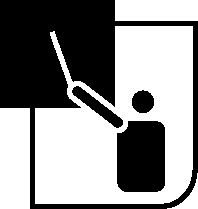
\includegraphics[width=0.75cm]{col11305.imgs/summary_presentation.png} &   \end{array} $ \hspace{2 pt}\raisebox{-5 pt}{} {(section shortcode: P10017 )} \par 
    \label{m38730*cid5}
            \subsection{ The Kinetic Theory of Matter}
            \nopagebreak
      \label{m38730*id308618}The \textbf{kinetic theory of 
matter} helps us to explain why matter exists in different \textsl{phases} (i.e. solid, liquid and gas), and how matter 
can change from one phase to the next. The kinetic theory of matter also helps 
us to understand other properties of matter. It is important to realise that 
what we will go on to describe is only a \textsl{theory}. It cannot be proved beyond doubt, but the 
fact that it helps us to explain our observations of changes in phase, and other 
properties of matter, suggests that it probably is more than just a theory.
\par 
      \label{m38730*id308641}Broadly, the Kinetic Theory of Matter says that:
\par 
      \label{m38730*id308647}\begin{itemize}[noitemsep]
            \label{m38730*uid34}\item Matter is made up of \textbf{particles} 
that are constantly moving.
\label{m38730*uid35}\item All particles have \textbf{energy}, but the energy varies depending on whether the 
substance is a solid, liquid or gas. Solid particles have the least amount of 
energy and gas particles have the greatest amount of energy.
\label{m38730*uid36}\item The \textbf{temperature} of a 
substance is a measure of the \textsl{average kinetic 
energy} of the particles.
\label{m38730*uid37}\item A change in \textbf{phase} 
may occur when the energy of the particles is changed.
\label{m38730*uid38}\item There are \textbf{spaces} 
between the particles of matter.
\label{m38730*uid39}\item There are \textbf{attractive 
forces} between particles and these become stronger as the particles 
move closer together. These attractive forces will either be intramolecular 
forces (if the particles are atoms) or intermolecular forces (if the particles 
are molecules). When the particles are extremely close, repulsive forces start 
to act.
\end{itemize}
      \label{m38730*id308767}Table 2.4 summarises the 
characteristics of the particles that are in each phase of matter.\par 
    % \textbf{m38730*uid40}\par
          \begin{table}[H]
    % \begin{table}[H]
    % \\ '' '0'
        \begin{center}
      \label{m38730*uid40}
      \begin{tabular}{|l|l|l|l|}\hline
\textbf{Property of matter} & \textbf{Solid} & \textbf{Liquid} & \textbf{Gas} \\ \hline
Particles & Atoms or molecules & Atoms or molecules & Atoms or molecules \\ \hline
Energy and movement of particles & Low energy - particles vibrate around a fixed point & Particles have less energy than in the gas phase & Particles have high energy and are constantly moving \\ \hline
Spaces between particles & Very little space between particles. Particles are tightly packed together & Smaller spaces than in gases, but larger spaces than in solids & Large spaces because of high energy \\ \hline
Attractive forces between particles & Very strong forces. Solids have a fixed volume. & Stronger forces than in gas. Liquids can be poured. & Weak forces because of the large distance between particles \\ \hline
Changes in phase & Solids become liquids if their temperature is increased. In some cases a solid may become a gas if the temperature is increased. & A liquid becomes a gas if its temperature is increased. It becomes a solid if its temperature decreases. & In general a gas becomes a liquid when it is cooled. (In a few cases a gas becomes a solid when cooled). Particles have less energy and therefore move closer together so that the attractive forces become stronger, and the gas becomes a liquid (or a solid.) \\ \hline
    \end{tabular}
      \end{center}
    \begin{caption} Table summarising the general features of solids, liquids and gases. \end{caption}
\end{table}

    \par
      \label{m38730*eip-933}The following presentation is a brief summary of the above. Try to fill in the blank spaces before clicking onto the next slide.
    \setcounter{subfigure}{0}
	\begin{figure}[H] % horizontal\label{m38730*slidesharefigure}
    \label{m38730*slidesharemedia}\label{m38730*slideshareflash}\raisebox{-5 pt}{ 
\includegraphics[width=0.5cm]{col11305.imgs/summary_www.png}} { (Presentation:  P10018 )}
      \vspace{2pt}
    \vspace{.1in}
 \end{figure}       \par \label{m38730*id309036}Let's look at an example that 
involves the three phases of water: ice (solid), water (liquid) and water vapour 
(gas). Note that in the Figure~2.3 below the 
molecules in the solid phase are represented by single spheres, but they would 
in reality look like the molecules in the liquid and gas phase. Sometimes we 
represent molecules as single spheres in the solid phase to emphasise the small 
amount of space between them and to make the drawing simpler.\par 
    \setcounter{subfigure}{0}
	\begin{figure}[H] % horizontal\label{m38730*uid41}
    \begin{center}
    \rule[.1in]{\figurerulewidth}{.005in} \\
        \label{m38730*uid41!!!underscore!!!media}\label{m38730*uid41!!!underscore!!!printimage}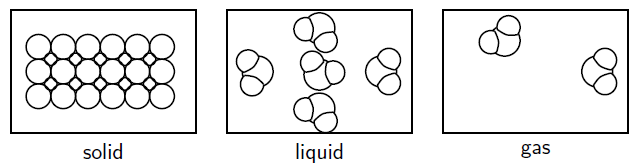
\includegraphics[width=8cm]{col11305.imgs/m38730_CG10C2_008.png} % m38730;CG10C2\_008.png;;;6.0;8.5;
      \vspace{2pt}
    \vspace{\rubberspace}\par \begin{cnxcaption}
	  \small \textbf{Figure 2.3: }The three phases of matter
	\end{cnxcaption}
    \vspace{.1in}
    \rule[.1in]{\figurerulewidth}{.005in} \\
    \end{center}
 \end{figure}       
      \label{m38730*id309053}Taking water as an example we find that in the solid 
phase the water molecules have very little energy and can't move away from each 
other. The molecules are held closely together in a regular pattern called a 
\textsl{lattice}. If the ice is heated, the energy 
of the molecules increases. This means that some of the water molecules are able 
to overcome the intermolecular forces that are holding them together, and the 
molecules move further apart to form \textsl{liquid 
water}. This is why liquid water is able to flow, because the 
molecules are more free to move than they were in the solid lattice. If the 
molecules are heated further, the liquid water will become water vapour, which 
is a gas. Gas particles have lots of energy and are far away from each other. 
That is why it is difficult to keep a gas in a specific area! The attractive 
forces between the particles are very weak and they are only loosely held 
together. Figure~2.4 shows the changes in phase that may occur in 
matter, and the names that describe these processes.\par 
    \setcounter{subfigure}{0}
	\begin{figure}[H] % horizontal\label{m38730*uid42}
    \begin{center}
    \rule[.1in]{\figurerulewidth}{.005in} \\
        \label{m38730*uid42!!!underscore!!!media}\label{m38730*uid42!!!underscore!!!printimage}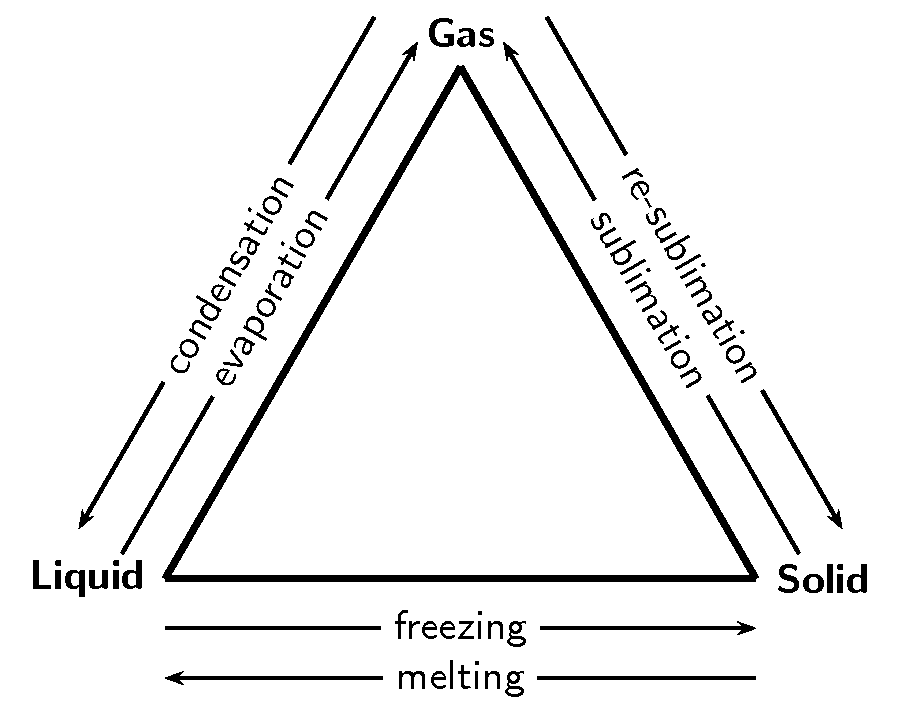
\includegraphics{col11305.imgs/m38730_CG10C2_009.png} % m38730;CG10C2\_009.png;;;6.0;8.5;
      \vspace{2pt}
    \vspace{\rubberspace}\par \begin{cnxcaption}
	  \small \textbf{Figure 2.4: }Changes in phase
	\end{cnxcaption}
    \vspace{.1in}
    \rule[.1in]{\figurerulewidth}{.005in} \\
    \end{center}
 \end{figure}       
\label{m38730*cid7}
            \subsection{ Summary}
            \nopagebreak
\label{m38730*id311034}\begin{itemize}[noitemsep]
            \label{m38730*id973}\item There are three states of matter: solid, liquid and gas.\label{m38730*id872}\item Diffusion is the movement of particles from a high concentration to a low concentration. Brownian motion is the diffusion of many particles.\label{m38730*uid80}\item The \textbf{kinetic theory of 
matter} attempts to explain the behaviour of matter in different 
phases.
\label{m38730*uid81}\item The kinetic theory of matter says that all matter is 
composed of \textbf{particles} which have a certain 
amount of \textbf{energy} which allows them to 
\textbf{move} at different speeds depending on the 
temperature (energy). There are \textbf{spaces} 
between the particles and also \textbf{attractive 
forces} between particles when they come close together.
\label{m38730*id643}\item Intramolecular force is the force between the atoms of a molecule, which holds 
them together. Intermolecular force is a force between molecules, which holds them together. \label{m38730*uid82}\item Understanding chemical bonds, intermolecular forces and 
the kinetic theory of matter can help to explain many of the \textbf{macroscopic properties} of matter.
\label{m38730*uid83}\item \textbf{Melting point} is the 
temperature at which a \textsl{solid} changes its 
phase to become a \textsl{liquid}. The reverse 
process (change in phase from liquid to solid) is called \textbf{freezing}. The stronger the chemical bonds and 
intermolecular forces in a substance, the higher the melting point will be.
\label{m38730*uid84}\item \textbf{Boiling point} is the 
temperature at which a liquid changes phase to become a gas. The reverse 
process (change in phase from gas to liquid) is called \textbf{condensing}. The stronger the 
chemical bonds and intermolecular forces in a substance, the higher the boiling 
point will be.
\label{m38730*uid85}\item \textbf{Density} is a measure 
of the mass of a substance per unit volume.
\label{m38730*uid86}\item \textbf{Viscosity} is a 
measure of how resistant a liquid is to flowing.
\end{itemize}
\label{m38730*cid9}
            \subsection{ End of chapter exercises}
            \nopagebreak
\label{m38730*id311490}\begin{enumerate}[noitemsep, label=\textbf{\arabic*}. ] 
            \label{m38730*uid87}\item Give one word or term for each of the following 
descriptions.
\label{m38730*id311506}\begin{enumerate}[noitemsep, label=\textbf{\alph*}. ] 
            \label{m38730*uid88}\item The 
property that determines how easily a liquid flows.
\label{m38730*uid89}\item The change in phase from liquid to gas.
\end{enumerate}
\label{m38730*uid92}\item If one substance A has a melting point that is \textsl{lower} than the melting point of substance B, this 
suggests that...
\label{m38730*id311675}\begin{enumerate}[noitemsep, label=\textbf{\alph*}. ] 
            \label{m38730*uid99}\item A 
will be a liquid at room temperature.
\label{m38730*uid100}\item The chemical bonds in substance A are weaker than those 
in substance B.
\label{m38730*uid101}\item The chemical bonds in substance A are stronger than 
those in substance B.
\label{m38730*uid102}\item B will be a gas at room temperature.
\end{enumerate}
                \label{m38730*uid103}\item Boiling point is an important concept to understand.
\label{m38730*id311744}\begin{enumerate}[noitemsep, label=\textbf{\alph*}. ] 
            \label{m38730*uid104}\item Define 'boiling point'.
\label{m38730*uid105}\item What change in phase takes place when a liquid reaches 
its boiling point?
\label{m38730*uid106}\item What is the boiling point of water?
\label{m38730*uid107}\item Use the kinetic theory of matter and your knowledge of 
intermolecular forces to explain why water changes phase at this temperature.
\end{enumerate}
\label{m38730*id762}\item Describe a solid in terms of the kinetic molecular theory. \newline
            \label{m38730*uid108}\item Refer to the table below which gives the melting and 
boiling points of a number of elements and then answer the questions that 
follow. (\textsl{Data from 
http://www.chemicalelements.com})
    % \textbf{m38730*id311817}\par
          \begin{table}[H]
    % \begin{table}[H]
    % \\ 'id2883166' '1'
        \begin{center}
      \label{m38730*id311817}
    \noindent
    \tabletail{%
        \hline
        \multicolumn{3}{|p{\mytableboxwidth}|}{\raggedleft \small \sl continued on next page}\\
        \hline
      }
      \tablelasttail{}
      \begin{xtabular}[t]{|l|l|l|}\hline
        \textbf{Element} &
        \textbf{Melting 
point} &
        \textbf{Boiling point (${}^{\ensuremath{{\,}^{\circ}}}\mathrm{C}$)}
% make-rowspan-placeholders
     \tabularnewline\cline{1-1}\cline{2-2}\cline{3-3}
      %--------------------------------------------------------------------
        copper &
        1083 &
        2567% make-rowspan-placeholders
     \tabularnewline\cline{1-1}\cline{2-2}\cline{3-3}
      %--------------------------------------------------------------------
        magnesium &
        650 &
        1107% make-rowspan-placeholders
     \tabularnewline\cline{1-1}\cline{2-2}\cline{3-3}
      %--------------------------------------------------------------------
        oxygen &
        -218,4 &
        -183% make-rowspan-placeholders
     \tabularnewline\cline{1-1}\cline{2-2}\cline{3-3}
      %--------------------------------------------------------------------
        carbon &
        3500 &
        4827% make-rowspan-placeholders
     \tabularnewline\cline{1-1}\cline{2-2}\cline{3-3}
      %--------------------------------------------------------------------
        helium &
        -272 &
        -268,6% make-rowspan-placeholders
     \tabularnewline\cline{1-1}\cline{2-2}\cline{3-3}
      %--------------------------------------------------------------------
        sulphur &
        112,8 &
        444,6% make-rowspan-placeholders
     \tabularnewline\cline{1-1}\cline{2-2}\cline{3-3}
      %--------------------------------------------------------------------
    \end{xtabular}
      \end{center}
\end{table}
    \par
  \label{m38730*id312057}\begin{enumerate}[noitemsep, label=\textbf{\alph*}. ] 
            \label{m38730*uid109}\item What state of matter (i.e. solid, liquid or gas) will each of 
these elements be in at room temperature?
\label{m38730*uid110}\item Which of these elements has the strongest forces 
between its atoms? Give a reason for your answer.
\label{m38730*uid111}\item Which of these elements has the weakest forces between 
its atoms? Give a reason for your answer.
\end{enumerate}
                \end{enumerate}
\label{m38730**end}
  \label{3fc6acf7f608d0b0e2d136d6a7710402**end}
\par \raisebox{-5 pt}{
\includegraphics[width=0.5cm]{col11305.imgs/summary_www.png}} Find the answers with the shortcodes:
 \par \begin{tabular}[h]{cccccc}
 (1.) l2t  &  (2.) lip  &  (3.) lim  &  (4.) lgf  &  (5.) liy  & \end{tabular}
